\documentclass{article}

\usepackage[english]{babel}     
\usepackage[utf8]{inputenc}     % accent symbols
\usepackage[T1]{fontenc}
\usepackage{lmodern}
\usepackage{microtype}
\usepackage{natbib}
\usepackage{tocbibind}          
\usepackage{amsmath}            % math symbols
\usepackage{amsthm}             % math symbols
\usepackage[colorlinks=true,linkcolor=red]{hyperref} % hyper link

% for code
\usepackage{listings}
\usepackage{color,xcolor}
\definecolor{mygreen}{rgb}{0,0.6,0}
\definecolor{mygray}{rgb}{0.9,0.9,0.9}
\definecolor{mymauve}{rgb}{0.58,0,0.82}
\lstset{
backgroundcolor=\color{mygray},
numbers=left,                    
columns=fullflexible,
breaklines=true,      
captionpos=b,         
tabsize=4,            
commentstyle=\color{mygreen}, 
escapeinside={\%*}{*)},       
keywordstyle=\color{blue},    
% stringstyle=\color{mymauve}\monaco,
frame=single,                        
rulesepcolor=\color{red!20!green!20!blue!20},
% identifierstyle=\color{red},
%% language=c++,
basicstyle=\tiny
}

\usepackage{indentfirst}
\setlength{\parindent}{2em}
\usepackage[onehalfspacing]{setspace}
% graph
\usepackage{pdfpages}
\usepackage{graphicx}
% box
\usepackage{booktabs}
\usepackage{tcolorbox}

%% user defined command
\newcommand{\keyword}[1]{\textbf{#1}}
\newcommand{\keywords}[1]{\textbf{#1}}
\newcommand{\lcmd}[1]{\texttt{#1}}
\newcommand{\head}[1]{\textnormal{\textbf{#1}}}
\newcommand{\itwords}[1]{\textit{#1}}

\usepackage{float}
% all symbols
\usepackage{tipa}
\usepackage{tipx}

\usepackage{datetime}
% \usepackage{movie15}


% variable
% TODO
\newcommand{\pdfauthor}{Mike Chyson (Li Mingming)}
\newcommand{\pdftitle}{Principles of Economics}
\newcommand{\pdfsubject}{Principles of Economics}
\newcommand{\pdfkeywords}{Principles of Economics}
\newcommand{\bookname}{Principles of Economics}
\newcommand{\bookoneword}{Citation and interpreation of principles of economics}
\newcommand{\timeandcompany}{Dec, 5, 2020}

\usepackage{bm}
\usepackage{amsfonts}

\begin{document}
\title{Coding Interview Strategy}
\maketitle{}
\newpage{}


\section{The Interview Process}

\subsection{The Basics}

\subsubsection{Do I need to know this "big O" stuff?}

Well, it depends. There are different types of interviews.

There’s the classic algorithmic coding interview, sometimes called the “Google-style whiteboard interview.” It’s focused on data structures and algorithms (queues and stacks, binary search, etc).


For startups and smaller shops, it’s a mixed bag. Most will ask at least a few algorithmic questions. But they might also include some role-specific stuff, like Java questions or SQL questions for a backend web engineer. They’ll be especially interested in your ability to ship code without much direction. You might end up doing a code test or pair-programming exercise instead of a whiteboarding session.


To make sure you study for the right stuff, you should ask your recruiter what to expect. Send an email with a question like, “Is this interview going to cover data structures and algorithms? Or will it be more focused around coding in X language.” They’ll be happy to tell you.

\subsubsection{Which programming language should I use?}

Companies usually let you choose, in which case you should use your most comfortable language. If you know a bunch of languages, prefer one that lets you express more with fewer characters and fewer lines of code, like Python or Ruby. It keeps your whiteboard cleaner.


\subsubsection{What should I wear?}

A good rule of thumb is to dress a tiny step above what people normally wear to the office.

\subsubsection{Should I send a thank-you note?}

Thank-you notes are nice, but they aren’t really expected. Be casual if you send one. No need for a hand-calligraphed note on fancy stationery. Opt for a short email to your recruiter or the hiring manager. Thank them for helping you through the process, and ask them to relay your thanks to your interviewers.


\subsection{Impostor Syndrome}

\begin{verbatim}
“It's a fluke that I got this job interview...”

“I studied for weeks, but I’m still not prepared...”

“I’m not actually good at this. They’re going to see right through me...”
\end{verbatim}

If any of these thoughts resonate with you, you're not alone. They are so common they have a name: impostor syndrome.

It’s that feeling like you’re on the verge of being exposed for what you really are—an impostor. A fraud.

\important{Impostor syndrome is like kryptonite to coding interviews.} It makes you give up and go silent.

You might stop asking clarifying questions because you’re afraid they’ll sound too basic. Or you might neglect to think out loud at the whiteboard, fearing you’ll say something wrong and sound incompetent.

You know you should speak up, but the fear of looking like an impostor makes that really, really hard.

\important{Here’s the good news: you’re not an impostor.} You just feel like an impostor because of some common cognitive biases about learning and knowledge.

Once you understand these cognitive biases—where they come from and how they work—you can slowly fix them. You can quiet your worries about being an impostor and keep those negative thoughts from affecting your interviews.


\subsubsection{Everything you could know}

Here’s how impostor syndrome works.

Software engineering is a massive field. There’s a huge universe of things you could know. Huge. Shown in Figure \ref{fig:you-could-know}.

\begin{figure}[!ht]
  \centering
  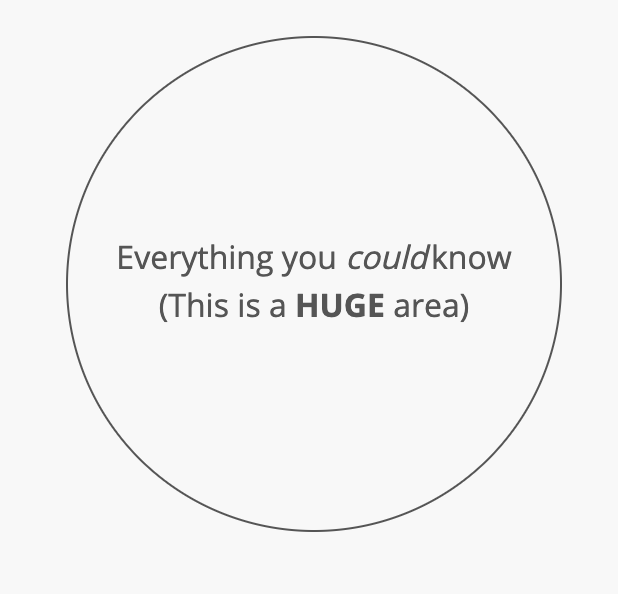
\includegraphics[width=0.5\textwidth]{pics/you-could-know}
  \caption{Everything you should know}
  \label{fig:you-could-know}
\end{figure}


In comparison to the vast world of things you could know, the stuff you actually know is just a tiny sliver. Shown in Figure \ref{fig:you-do-know}.

\begin{figure}[!ht]
  \centering
  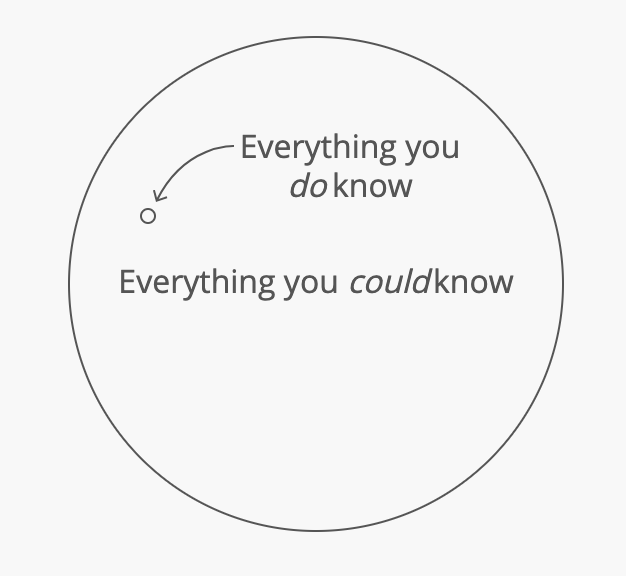
\includegraphics[width=0.5\textwidth]{pics/you-do-know}
  \caption{Everything you do know}
  \label{fig:you-do-know}
\end{figure}

 

That’s the first problem. \important{It feels like you don’t really know that much, because you only know a tiny sliver of all the stuff there is to know.}


\subsubsection{The expanding universe}

It gets worse: \important{counterintuitively, as you learn more, your sliver of knowledge feels like it's shrinking.}

That's because you brush up against more and more things you don’t know yet. Whole disciplines like machine learning, theory of computation, and embedded systems. Things you can't just pick up in an afternoon. Heavy bodies of knowledge that take months to understand.

So the universe of things you could know seems to keep expanding faster and faster—much faster than your tiny sliver of knowledge is growing. It feels like you'll never be able to keep up.


\subsubsection{What everyone else knows}

Here's another common cognitive bias: we assume that because something is easy for us, it must be easy for everyone else. So when we look at our own skills, we assume they're not unique. But when we look at other people's skills, we notice the skills they have that we don't have.

The result? We think everyone’s knowledge is a superset of our own (Figure \ref{fig:false-what-everyone-else-know}):

\begin{figure}[!ht]
  \centering
  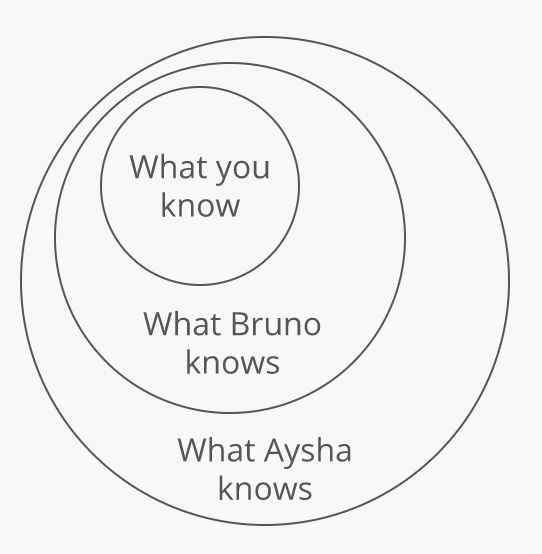
\includegraphics[width=0.5\textwidth]{pics/false-what-everyone-else-know}
  \label{fig:false-what-everyone-else-know}
\end{figure}


This makes us feel like everyone else is ahead of us. Like we're always a step behind.

But the truth is more like this (Figure \ref{fig:true-what-everyone-else-know}):

\begin{figure}[!ht]
  \centering
  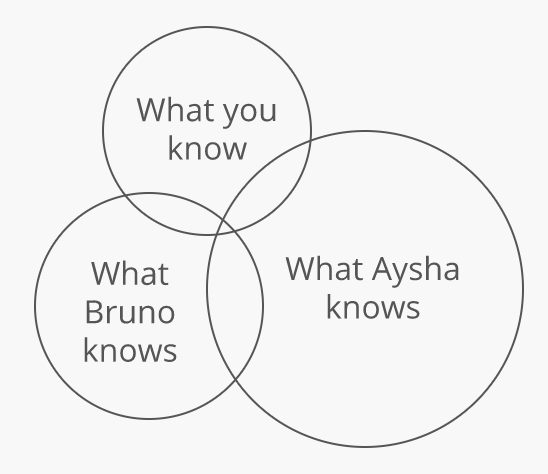
\includegraphics[width=0.5\textwidth]{pics/true-what-everyone-else-know}
  \label{fig:true-what-everyone-else-know}
\end{figure}


There's a whole area of stuff you know that neither Aysha nor Bruno knows. An area you're probably blind to, because you're so focused on the stuff you don't know.


\subsubsection{It's a problem of focus}

Focusing on what you don't know causes you to underestimate what you do know. And that's what causes impostor syndrome.

By looking at the vast (and expanding) universe of things you could know, you feel like you hardly know anything.

And by looking at what Aysha and Bruno know that you don't know, you feel like you're a step behind.

And interviews make you really focus on what you don't know. You focus on what could go wrong. The knowledge gaps your interviewers might find. The questions you might not know how to answer.

But remember:

Just because Aysha and Bruno know some things you don't know, doesn't mean you don't also know things Aysha and Bruno don't know.

And more importantly, everyone's body of knowledge is just a teeny-tiny sliver of everything they could learn. We all have gaps in our knowledge. We all have interview questions we won't be able to answer.

You're not a step behind. You just have a lot of stuff you don't know yet. Just like everyone else.

\end{document}

